\chapter{Introducción específica}

En este capítulo se presenta un resumen de los conceptos más relevantes acerca de la red TCN y su implementación en las formaciones de Trenes Argentinos, y se detallan las diferentes tecnologías utilizadas para el desarrollo del dispositivo de captura.

\section{La red TCN}

La red TCN es una combinación jerárquica de dos buses de datos para transmitir información dentro de una formación ferroviaria. El Multifunction Vehicle Bus (MVB) interconecta los diferentes dispositivos presentes dentro de cada vehículo, y el Wire Train Bus (WTB) interconecta los diferentes vehículos. Los componentes de la red TCN están estandarizados en la norma IEC 61375-1.

\begin{figure}[htbp]
	\centering
	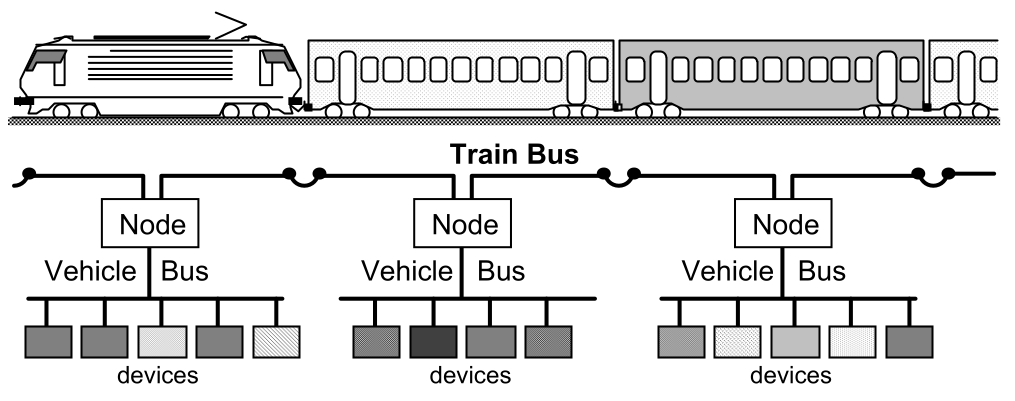
\includegraphics[width=.8\textwidth]{./Figures/tcn-mvb-wtb.png}
	\caption[Wire Train Bus y Multifunction Vehicle Bus]{Wire Train Bus y Multifunction Vehicle Bus.
        \\ \todo{CAMBIAR: La imagen original tiene copyright.}}
\end{figure}

Dado que el dispositivo desarrollado se conecta al bus MVB, a continuación se exponen las características principales de este bus de comunicación.

\subsection{El bus MVB}

El bus MVB interconecta diferentes dispositivos ubicados en el mismo vehículo o en diferentes vehículos. Proporciona tanto la interconexión de equipos programables entre sí como la interconexión de estos equipos con sus sensores y actuadores. El MVB puede direccionar hasta 4095 dispositivos, y puede funcionar como \textit{train bus} en segmentos en los que los vehículos no son separados durante su operación normal (abarcando de esta manera más de un vehículo).

\subsection{Capa física MVB}

El bus MVB ofrece tres opciones para la capa física:

\begin{itemize}
\item El medio Electrical Short Distance (ESD), para distancias de hasta 20~m, que soporta hasta 32 dispositivos por segmento, con transceptores de tipo RS-485.
\item El medio Electrical Middle Distance (EMD), para distancias de hasta 200~m, que soporta hasta  32 dispositivos por segmento, con transformadores y transceptores compatibles con la norma IEC 61158-2 \cite{iec61158_2}.
\item El medio Optical Glass Fibre (OGF), para distancias de hasta 2000~m, y soporta conexiones punto a punto o subredes de topología tipo estrella.
\end{itemize}

Puede haber diferentes buses en un vehículo, interconectados mediante un \textit{gateway} al bus WTB, como se muestra en la fig.~\ref{fig:emd-esd-wtb}.
La norma recomienda el medio EMD para conectar vehículos que se acoplan y desacoplan con frecuencia en la vía.

\begin{figure}[htbp]
	\centering
	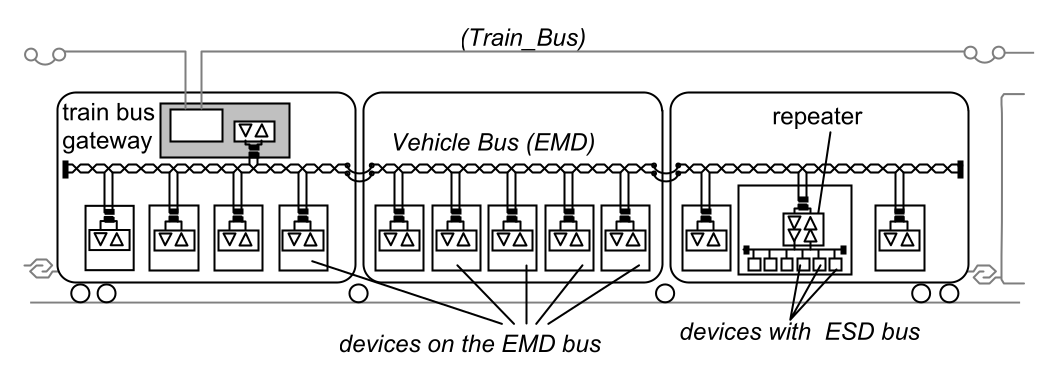
\includegraphics[width=1\textwidth]{./Figures/tcn-emd-esd-wtb.png}
	\caption[MVB abarcando tres vehículos]{MVB abarcando tres vehículos.
        \\ \todo{CAMBIAR: La imagen original tiene copyright.}}
    \label{fig:emd-esd-wtb}
\end{figure}

En algunas formaciones el bus MVB puede abarcar varios vehículos, y un segmento EMD puede abarcar hasta 200~m, lo que equivale a unos 5 vehículos, sin repetidores.
Como se muestra en la fig.~\ref{fig:segmento}, cada dispositivo conectado a un segmento EMD tiene dos conectores de tipo DB9 que van, respectivamente, al dispositivo anterior y siguiente en el segmento. Los dispositivos en los extremos del segmento tienen un terminador.
En la fig.~\ref{fig:db9} se muestra la configuración de pines de estos conectores, que conforman a la norma IEC 61158-2 de tipo 6 (RS-485).

\begin{figure}[htbp]
	\centering
	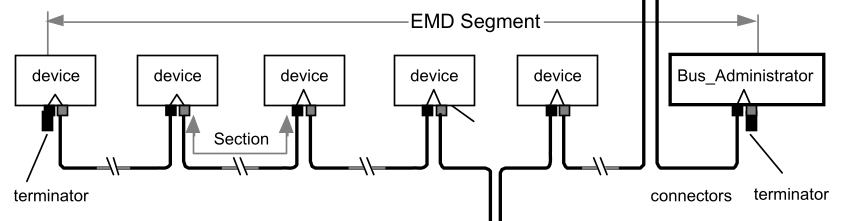
\includegraphics[width=1\textwidth]{./Figures/segmento.png}
	\caption[Un segmento EMD]{Un segmento EMD.
        \\ \todo{CAMBIAR: La imagen original tiene copyright.}}
    \label{fig:segmento}
\end{figure}

\begin{figure}[htbp]
	\centering
	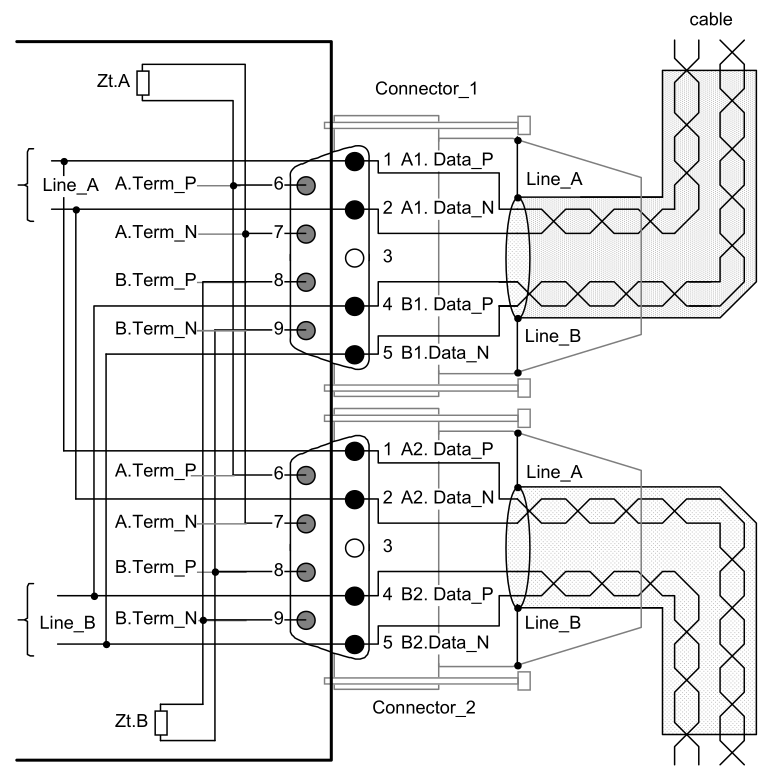
\includegraphics[width=0.8\textwidth]{./Figures/db9-emd.png}
	\caption[Configuración de pines del conector DB9 del medio EMD]{Configuración de pines del conector DB9 del medio EMD.
        \\ \todo{CAMBIAR: La imagen original tiene copyright.}}
    \label{fig:db9}
\end{figure}

Todos los medios MVB operan a una velocidad unificada de 1,5~Mbit/s.
La información se transmite utilizando una codificación Manchester, que combina en una única señal la información y el \textit{clock}.
Un ``1'' se transmite como una transición negativa en el medio de una celda de bit, y un ``0'' se transmite como una transición positiva.

\begin{figure}[htbp]
	\centering
	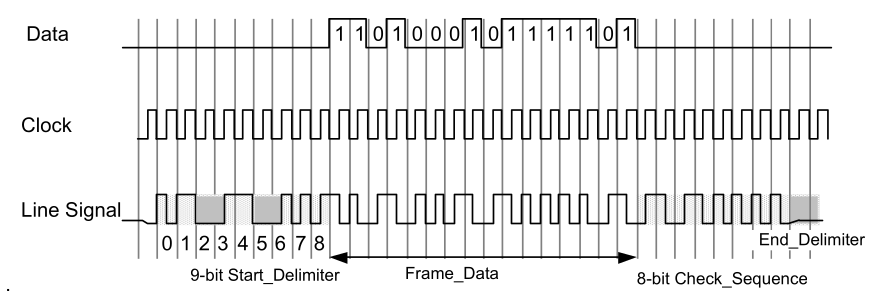
\includegraphics[width=1\textwidth]{./Figures/manchester.png}
	\caption[Delimitador de trama, información codificada con Manchester y la secuencia de verificación]{Delimitador de trama, información codificada con Manchester y la secuencia de verificación.
        \\ \todo{CAMBIAR: La imagen original tiene copyright.}}
\end{figure}

\subsection{Tramas MVB}

En el bus MVB se transmiten dos tipos de tramas:

\begin{itemize}
\item La trama \textit{master}, que es transmitida únicamente por el dispositivo maestro del bus.
\item La trama \textit{slave}, que es transmitida por un dispositivo esclavo en respuesta a una trama \textit{master}.
\end{itemize}

Ambos tipos de tramas son precedidas por un delimitador que marca el comienzo de la transmisión, y son sucedidas por una secuencia de verificación y un delimitador para marcar la finalización.

Una secuencia de una trama \textit{master} seguida de una trama \textit{slave} conforman un \textit{telegrama}.

\begin{figure}[htbp]
	\centering
	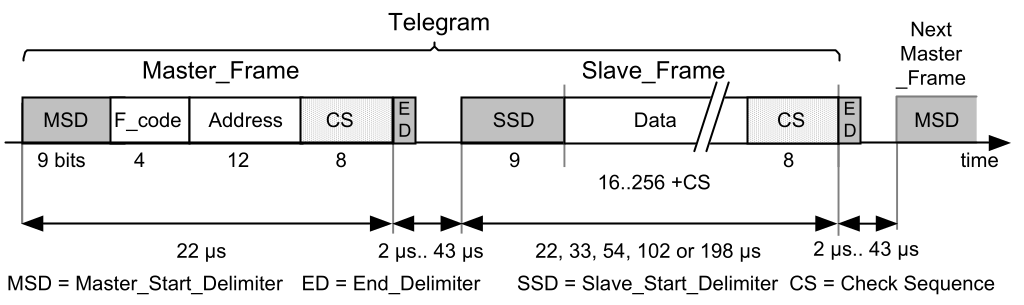
\includegraphics[width=1\textwidth]{./Figures/telegrama.png}
	\caption[Un telegrama MVB]{Un telegrama MVB.
        \\ \todo{CAMBIAR: La imagen original tiene copyright.}}
\end{figure}

Las tramas \textit{master} tienen una longitud fija de 16 bits (sin contar los delimitadores), e incluyen:

\begin{itemize}
\item Un código de 4 bits llamado \texttt{F\_code}, que indica el tipo y tamaño de la trama \textit{slave} esperada a continuación.
\item Un campo de 12 bits, que puede contener una dirección de destino, o parámetros específicos al \texttt{F\_code}.
\end{itemize}

Todos los dispositivos conectados al bus decodifican la trama \textit{master}. El dispositivo direccionado luego responde con su trama \textit{slave}, que a su vez puede ser recibida por otros dispositivos.
Las direcciones de los dispositivos se asignan durante la configuración de la red y no cambian durante la operación.

Son de particular interés las tramas con \texttt{F\_code = 0..4}. Este tipo de telegramas son denominados \texttt{Process\_Data}, y en este caso el campo de 12 bits contiene una dirección lógica que se interpreta como un \textit{puerto}. Cada puerto en el bus direcciona unívocamente una \textit{variable} en el bus, que puede contener uno o más valores como la velocidad actual, la tensión de red, el estado de las puertas, etc. Cada dispositivo \textit{slave} almacena uno o más puertos, y al ser direccionado responde con el valor actual de la variable correspondiente.

\section{TCN en las formaciones de Trenes Argentinos}

En la fig.~\ref{fig:tms} se muestra un diagrama de la topología de la red TCN en un segmento de una formación, compuesto por 3 vehículos EMU. Para el bus MVB se utiliza en este caso el medio físico EMD, y por lo tanto el dispositivo desarrollado en este trabajo es compatible con este medio.

\begin{figure}[htbp]
	\centering
	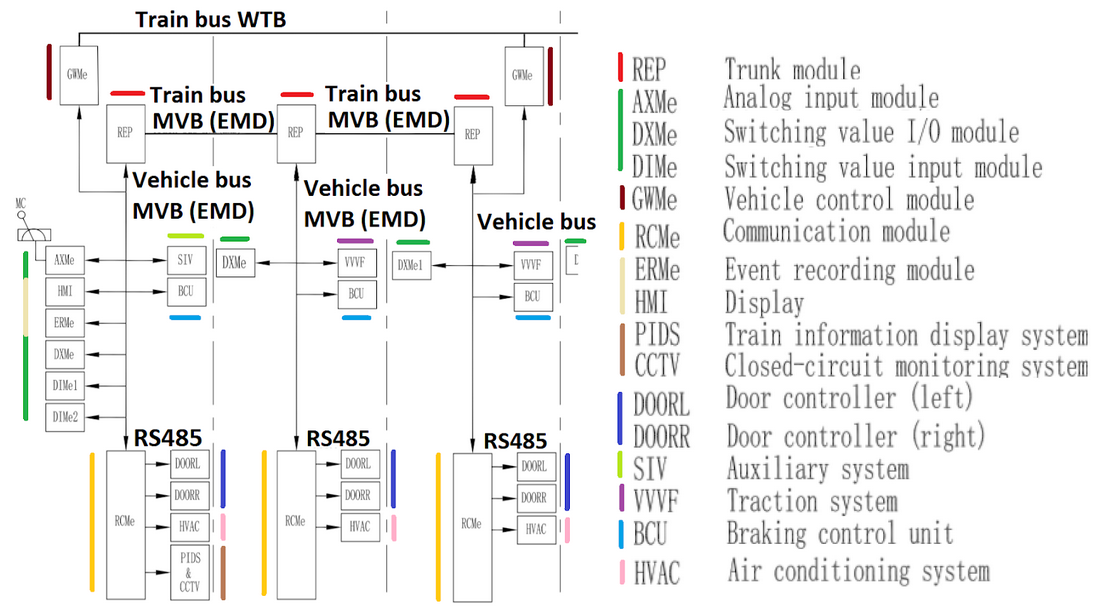
\includegraphics[width=1\textwidth]{./Figures/tms.png}
	\caption[Topología de la red TCN en una formación de Trenes Argentinos]{Topología de la red TCN en una formación de Trenes Argentinos.
        \\ \todo{REVISAR: Rehacer para mejorar la legibilidad.}}
    \label{fig:tms}
\end{figure}

En la fig.~\ref{fig:rcme} se muestra una fotografía del interior de un \textit{rack}, en la cabina del conductor de una formación de la línea Mitre. En la imagen se observa uno de los módulos conectados en el bus MVB, el módulo de comunicación RCMe, que a su vez controla las puertas (DOORR, DOORL), el sistema de aire acondicionado (HVAC) y el sistema de información al pasajero (PIDS). En el panel frontal del módulo RCMe, los conectores DB9 X1 y X2 corresponden al bus MVB.

\begin{figure}[htbp]
	\centering
	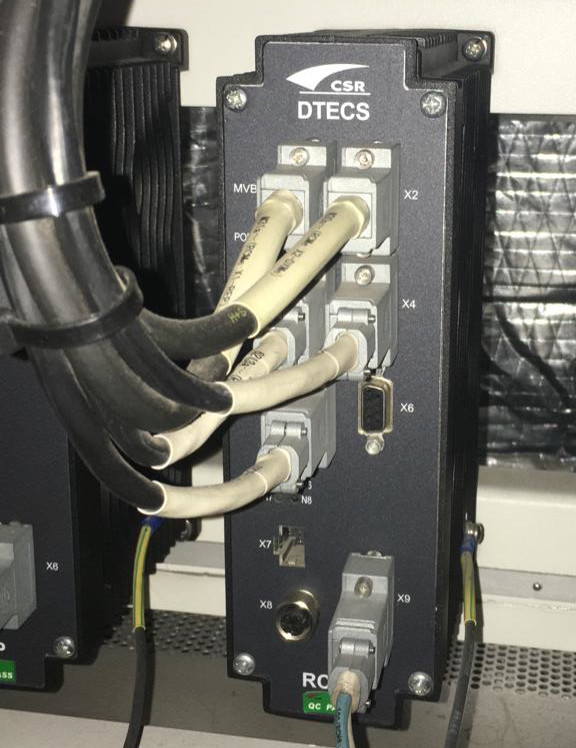
\includegraphics[width=0.5\textwidth]{./Figures/RCMe.jpeg}
	\caption[El módulo de comunicación RCMe]{El módulo de comunicación RCMe presente en un EMU.
        \\ \todo{REVISAR: Agregar indicaciones y una leyenda para cada conector.}}
    \label{fig:rcme}
\end{figure}

En la cabina del conductor, la pantalla HMI (Human Machine Interface) tiene un modo de operación en el que permite visualizar el valor de algunas variables que son transmitidas periódicamente en forma de \texttt{Process\_Data}. En la fig.~\ref{fig:hmi} se puede ver que en el puerto 0 hay una variable de 16 bits cuyo valor binario actual es 1100 0001 0110 0101, o 33702 si se interpreta como un número decimal.

\begin{figure}[htbp]
	\centering
	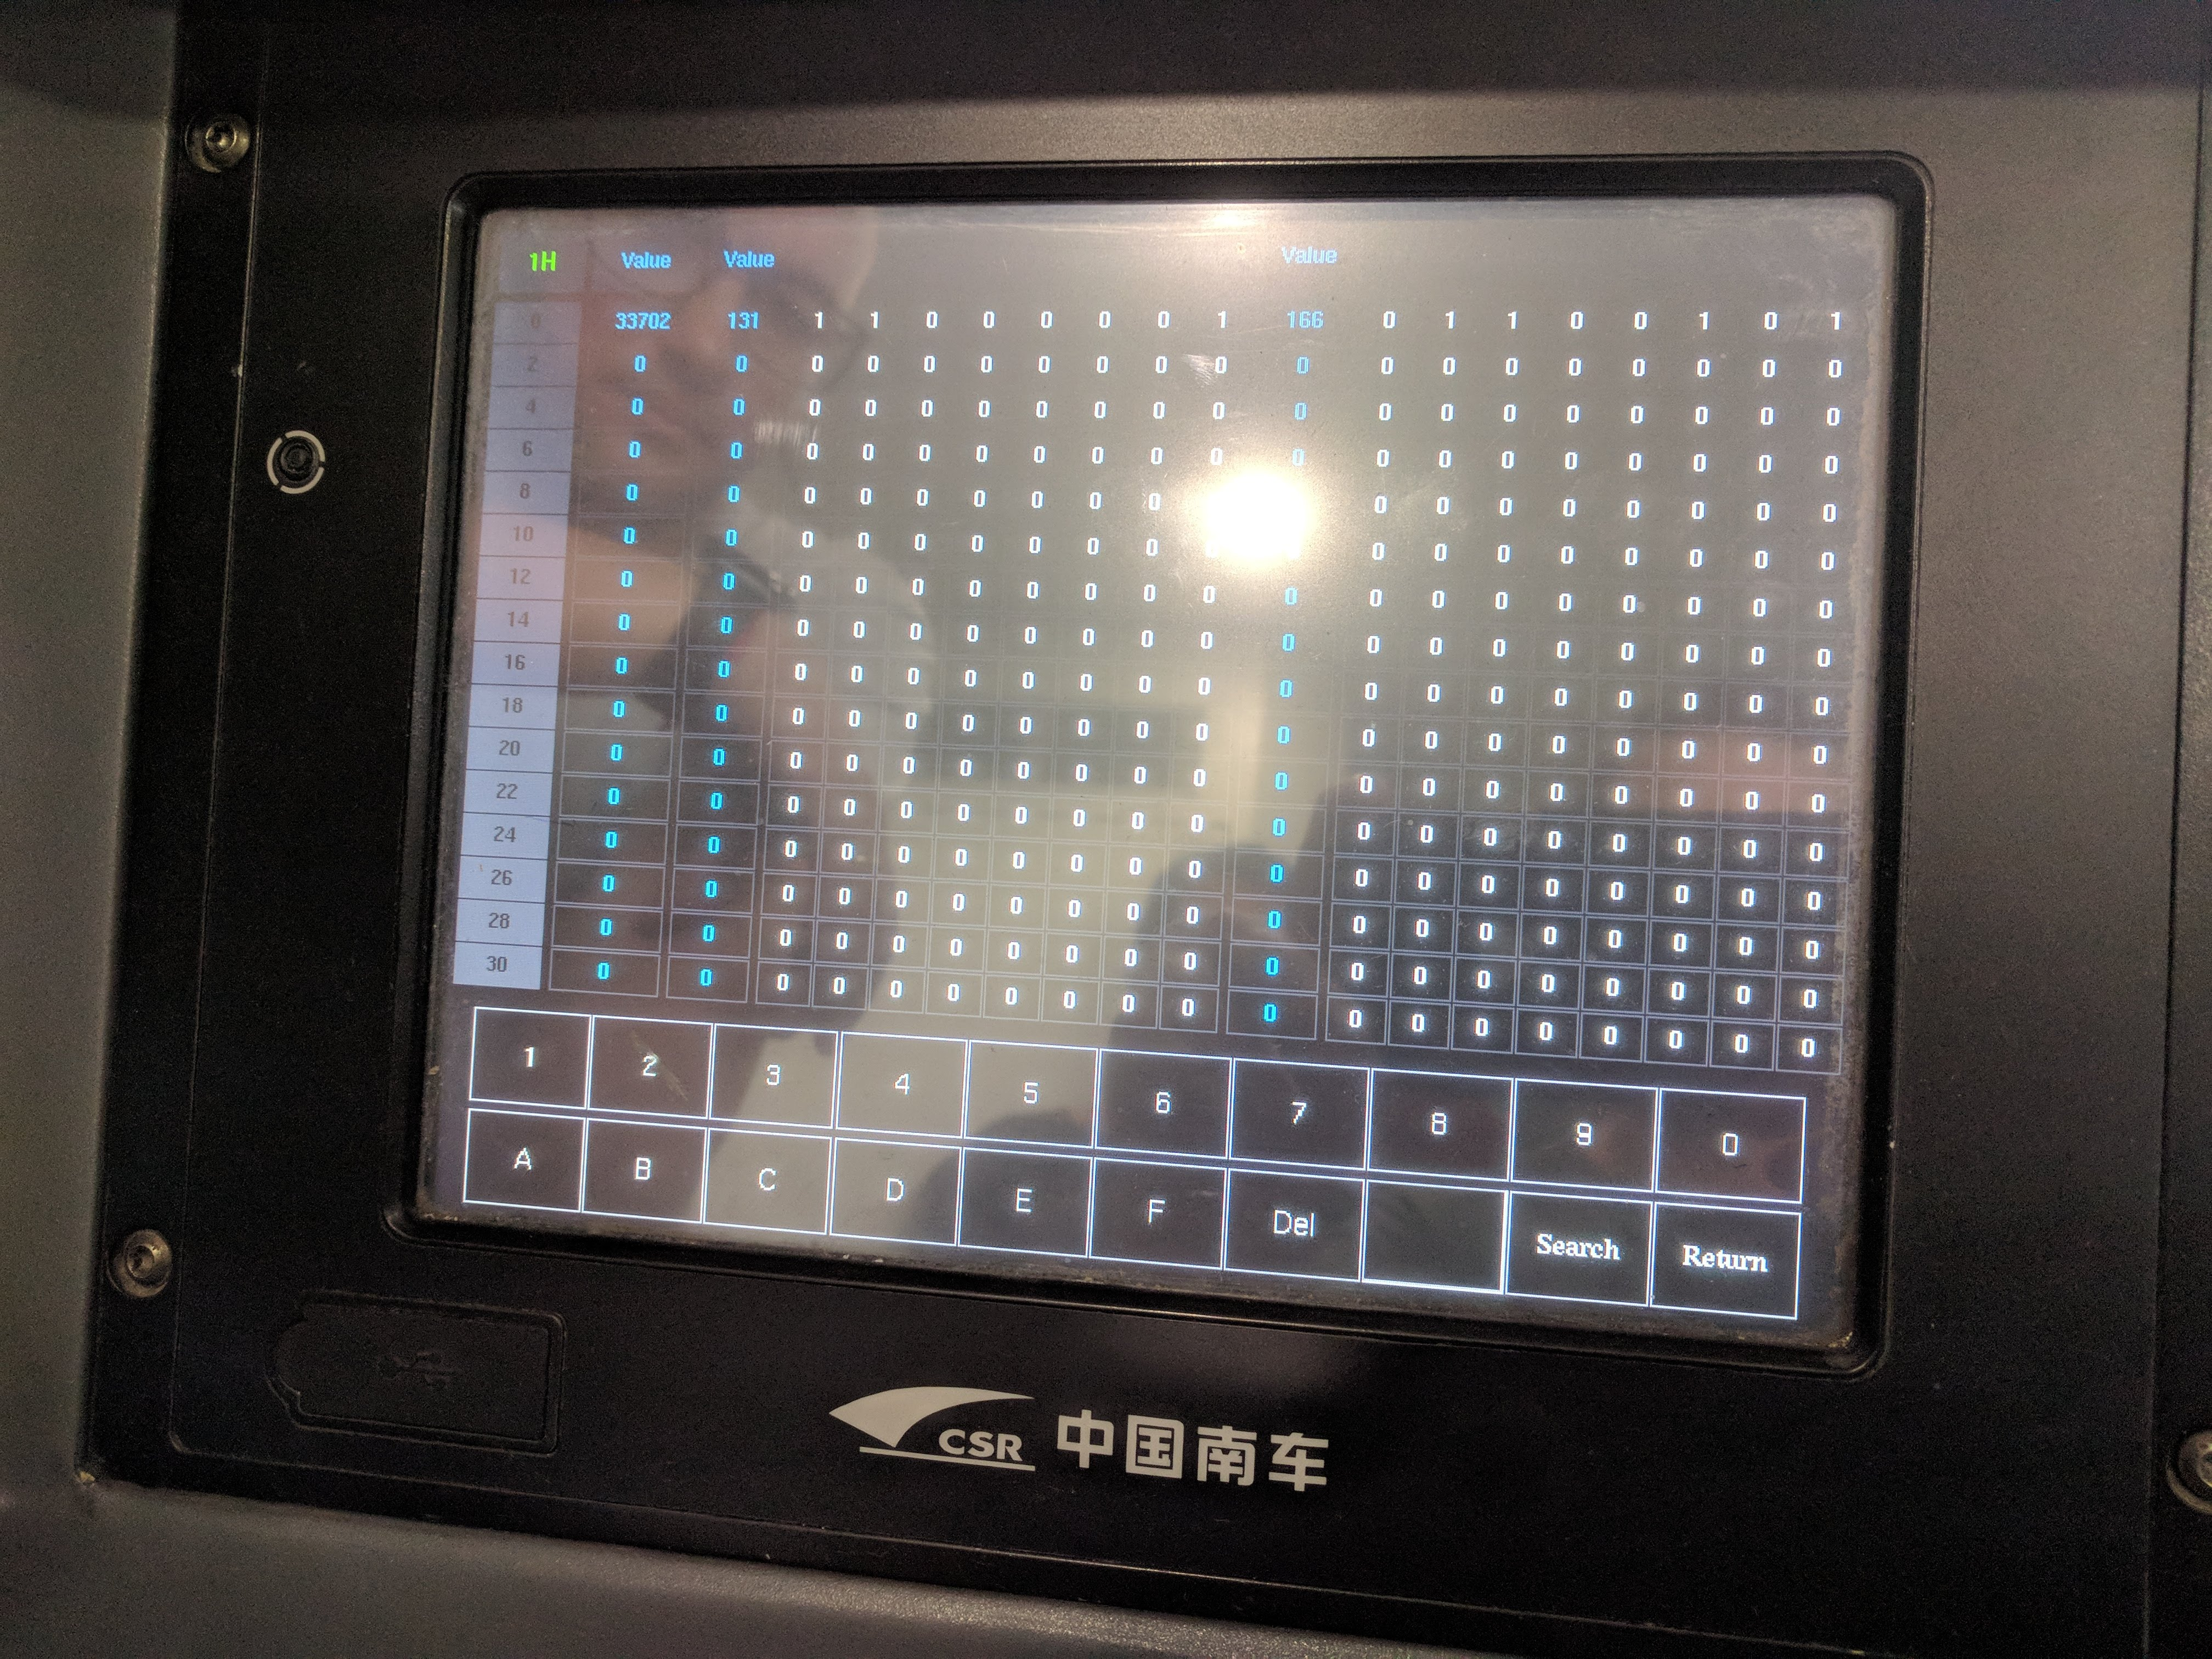
\includegraphics[width=1\textwidth]{./Figures/hmi.jpg}
	\caption[El HMI mostrando algunas variables]{El HMI mostrando algunas variables.}
    \label{fig:hmi}
\end{figure}



\section{Componentes del sistema}
